\begin{figure}[t!]
\centering

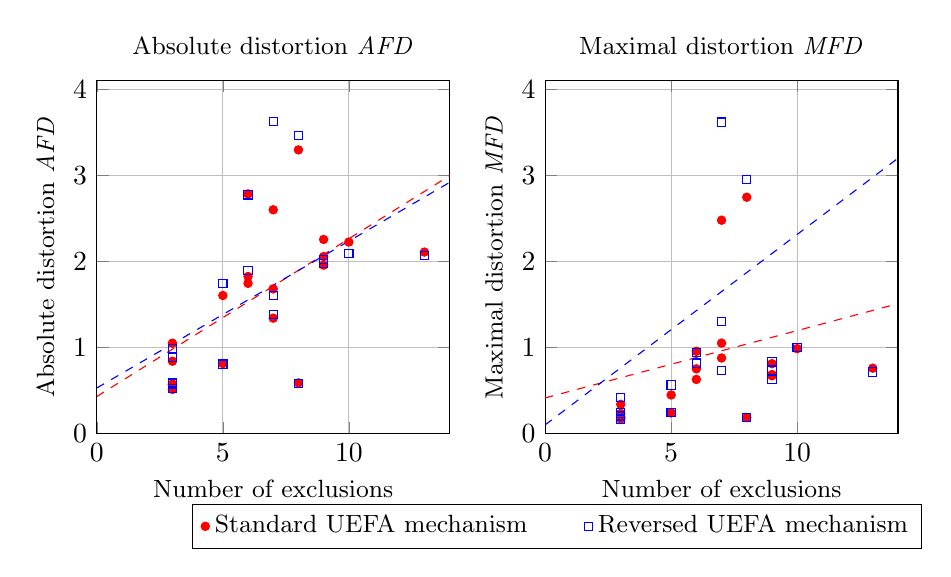
\begin{tikzpicture}
\begin{axis}[
name = axis1,
title = {Absolute distortion $\mathit{AFD}$},
title style = {font=\small},
xlabel = Number of exclusions,
x label style = {font=\small},
ylabel = Absolute distortion $\mathit{AFD}$,
y label style = {font=\small},
width = 0.5\textwidth,
height = 0.5\textwidth,
nodes near coords,
xmajorgrids = true,
ymajorgrids = true,
xmin = 0,
xmax = 14,
ymin = 0,
ymax = 4.1,
]
% Standard
\addplot [scatter,red,only marks,mark size=1.5pt,point meta=explicit symbolic] coordinates {
(3,1.04832279448298)
(6,2.78287689950249)
(3,0.839184282198522)
(5,0.811377006231495)
(6,1.82378600478088)
(10,2.22406950934172)
(3,0.571544174180777)
(5,1.60285124713845)
(3,0.57101108560184)
(6,1.74399211861615)
(8,0.587354304642073)
(7,1.67930541674952)
(3,0.512016244278464)
(9,1.95554048557555)
(7,2.59846861187892)
(9,2.2538359400523)
(13,2.10715692679413)
(9,2.05515532494286)
(7,1.33937602567988)
(8,3.29469615239078)
};
% Trend line
\draw[red,dashed] (\pgfkeysvalueof{/pgfplots/xmin},0.1833 * \pgfkeysvalueof{/pgfplots/xmin} + 0.4286) -- (\pgfkeysvalueof{/pgfplots/xmax},0.1833 * \pgfkeysvalueof{/pgfplots/xmax} + 0.4286);

% Reversed
\addplot [scatter,blue,only marks,mark=square,mark size=1.5pt,point meta=explicit symbolic] coordinates {
(3,0.989599020898075)
(6,2.77272162609176)
(3,0.882225922887611)
(5,0.804479536247259)
(6,1.89173619290457)
(10,2.09160762935801)
(3,0.587055198243915)
(5,1.74005987458943)
(3,0.519550231666842)
(6,1.89160499769357)
(8,0.581640971308739)
(7,1.38512771352651)
(3,0.576116745979197)
(9,1.97576352798896)
(7,3.62429179262455)
(9,1.97642062090336)
(13,2.06549367098018)
(9,2.0241129339814)
(7,1.60021187831083)
(8,3.46137598899209)
};
% Trend line
\draw[blue,dashed] (\pgfkeysvalueof{/pgfplots/xmin},0.176 * \pgfkeysvalueof{/pgfplots/xmin} + 0.528) -- (\pgfkeysvalueof{/pgfplots/xmax},0.176 * \pgfkeysvalueof{/pgfplots/xmax} + 0.4528);
\end{axis}

\begin{axis}[
at = {(axis1.south east)},
xshift = 0.1\textwidth,
title = {Maximal distortion $\mathit{MFD}$},
title style = {font=\small},label = Reversed UEFA mechanism,
xlabel = Number of exclusions,
x label style = {font=\small},
ylabel = Maximal distortion $\mathit{MFD}$,
y label style = {font=\small},
width = 0.5\textwidth,
height = 0.5\textwidth,
nodes near coords,
xmajorgrids = true,
ymajorgrids = true,
xmin = 0,
xmax = 14,
ymin = 0,
ymax = 4.1,
legend style = {font=\small,at={(-1,-0.2)},anchor=north west,legend columns=2},
legend entries = {Standard UEFA mechanism$\qquad$,Reversed UEFA mechanism},
]
% Standard
\addplot [scatter,red,only marks,mark size=1.5pt,point meta=explicit symbolic] coordinates {
(3,0.167207834827748)
(6,0.954354657084946)
(3,0.338294695652175)
(5,0.238726213373402)
(6,0.627172827546957)
(10,0.984714267737619)
(3,0.181931603254895)
(5,0.446758893401017)
(3,0.232209376626216)
(6,0.750775291231923)
(8,0.184253291392622)
(7,0.876386062001772)
(3,0.189567961080137)
(9,0.669658224507283)
(7,2.47753449551675)
(9,0.810602740660529)
(13,0.758046317682318)
(9,0.684134974281392)
(7,1.04947518510772)
(8,2.74443511455108)
};
% Trend line
\draw[red,dashed] (\pgfkeysvalueof{/pgfplots/xmin},0.0986 * \pgfkeysvalueof{/pgfplots/xmin} + 0.41271) -- (\pgfkeysvalueof{/pgfplots/xmax},0.0986 * \pgfkeysvalueof{/pgfplots/xmax} + 0.1271);

% Reversed
\addplot [scatter,blue,only marks,mark=square,mark size=1.5pt,point meta=explicit symbolic] coordinates {
(3,0.166188033034451)
(6,0.942906657084946)
(3,0.419310695652172)
(5,0.244454213373402)
(6,0.816824827546955)
(10,0.99677626773762)
(3,0.207653831977128)
(5,0.563012893401013)
(3,0.196529376626217)
(6,0.815580031850632)
(8,0.187393291392624)
(7,0.729732062001773)
(3,0.236607376626216)
(9,0.735236570694087)
(7,3.61684049551675)
(9,0.625820781808339)
(13,0.714800317682318)
(9,0.83265158850227)
(7,1.30230718510772)
(8,2.95202711455108)
};
% Trend line
\draw[blue,dashed] (\pgfkeysvalueof{/pgfplots/xmin},0.2213 * \pgfkeysvalueof{/pgfplots/xmin} + 0.099) -- (\pgfkeysvalueof{/pgfplots/xmax},0.2213 * \pgfkeysvalueof{/pgfplots/xmax} + 0.099);
\end{axis}
\end{tikzpicture}

\caption{Fairness distortions of the draw mechanisms in the UEFA \\ Champions League Round of 16 by the number of association constraints \\ \vspace{0.2cm}
\footnotesize{\emph{Note}: Dashed lines indicate fitted linear relationship.}}
\label{Fig2}

\end{figure}